\chapter{Ristrutturazione della progettazione concettuale}
    \section{Analisi della ristrutturazione del Diagramma ER}
        \subsection{Analisi delle ridondanze}
            Nel modello concettuale sono presenti attributi ridondanti. Tali attributi sono "Numero di afferenti" dell'entità "LABORATORIO", "Costo totale attrezzature" e "Costo totale contratti a progetto" dell'entità "PROGETTO", poiché attributi derivabili. Per risolvere le ridondanze, analizziamo separatamente il caso in cui scegliamo di mantenere la ridondanza e il caso in cui scegliamo di rimuoverla. Supponiamo di eseguire le seguenti operazioni:
            \begin{itemize}
                \item Registrazione delle afferenze di un dipendete indeterminato a uno o più laboratori. Visualizzazione di tutti i dati relativi a un laboratorio, circa 5 volte al mese.
                \item Acquisto di una nuova attrezzatura, indicandone il costo e il progetto tramite cui effettuiamo l'acquisto. Visualizzazione di tutti i dati relativi ad un progetto, circa 25 volte al mese.
                \item Assunzione di un nuovo dipendente con contratto a progetto, indicandone il costo del contratto e il progetto per cui lavorerà. Visualizzazione di tutti i dati relativi ad un progetto, circa 25 volte al mese, come nel caso delle attrezzature.
            \end{itemize}

            Tenendo conto del costo doppio degli accessi in scrittura rispetto agli accessi in lettura ed un uso di memoria molto ridotto a supporto degli attributi ridondanti, si può concludere che:
            \begin{itemize}
                \item Nel tipo di entità "LABORATORIO", con l'inserimento dell'attributo ridondante "Numero di afferenti", si ottiene un risparmio di circa la metà degli accessi mensili al database, considerando le operazioni precedentemente riportate.
                \item Nel tipo di entità "PROGETTO", con l'inserimento dell'attributo ridondante "Costo totale attrezzature", si ottiene un risparmio di circa poco meno della metà degli accessi mensili al database per le operazioni precedentemente riportate.
                \item Nel tipo di entità "PROGETTO", con l'inserimento dell'attributo ridondante "Costo totale contratti a progetto", si ottiene un risparmio di più della metà degli accessi mensili al database per le operazioni precedentemente riportate.
            \end{itemize}
            E' presente un'ulteriore ridondanza tra la sottoclasse "DIRIGENTE" della superclasse "DIPENDENTE CON CONTRATTO A TEMPO INDETERMINATO" e la sottoclasse "PROMOSSO A DIRIGENTE" dalla specializzazione dell'entità debole "SCATTO DI CARRIERA". Tale ridondanza viene mantenuta, facendo riferimento ai criteri già illustrati, per garantire una facilità di accesso ai dati ed un miglioramento delle prestazioni, anche se minimo.
            
            Inoltre, la relazione "LAVORARE" tra un laboratorio ed un progetto potrebbe sembrare una ridondanza, dato che se un laboratorio ha un'attrezzatura acquistata tramite i fondi di un progetto, di certo avrà lavorato a quel progetto. Tuttavia, senza la relazione "LAVORARE" non sarebbe possibile tenere traccia di eventuali laboratori che hanno lavorato a un progetto ma a cui non è stato assegnato alcuna attrezzatura acquistata tramite i fondi del progetto. In effetti, si potrebbe anche non acquistare alcuna attrezzatura tramite tali fondi.\\

        \subsection{Analisi degli identificativi}
            Per ognuno dei seguenti tipi di entità scegliamo gli identificativi:
            \begin{itemize}
                \item DIPENDENTE\\
                Scegliamo come identificativo l'attributo "Matricola", il quale assumiamo essere un codice alfanumerico di otto caratteri.
                Ad ogni dipendente sarà assegnata univocamente una matricola al momento dell'assunzione. Ogni matricola sarà diversa dalle altre ed identificherà un dipendente che lavora all'interno dell'azienda grazie al contratto di assunzione. Se il dipendente venisse licenziato e in seguito riassunto, riceverebbe una nuova matricola dovuta alla nuova assunzione con un contratto diverso.
                \item PROGETTO\\
                Scegliamo come identificativo l'attributo "CUP". Il CUP è un codice composto da quindici caratteri alfanumerici atto ad identificare univocamente un progetto.
                \item LABORATORIO\\
                Scegliamo come identificativo l'attributo "Nome", dato che all'interno di una singola azienda assumiamo che non venga assegnato ad un laboratorio un nome precedentemente assegnato ad altri laboratori.
                \item ATTREZZATURA\\
                Introduciamo come identificativo un attributo "idAttrezzatura", ovvero un codice numerico che identifica ogni attrezzatura acquistata.
            \end{itemize}

        \subsection{Rimozione degli attributi multivalore}
            Non abbiamo modellato alcuna situazione presentante attributi multivalore.
                
        \subsection{Rimozione degli attributi composti}
            L'unico attributo composto presente nel diagramma concettuale è l'attributo di "DIPENDENTE" chiamato "Indirizzo". Scegliamo di trattare tale attributo come attributo atomico, trascurando i vari attributi componenti semplici. Infatti supponiamo che l'azienda in questione avrà di rado bisogno di fare ricerche basate sugli indirizzi (oppure su informazioni ricavabili da essi), dato che la base di dati è modellata principalmente per la gestione dei laboratori, progetti e dipendenti di un'azienda.
                
        \subsection{Partizione/Accorpamento delle associazioni}
            Dal momento i tipi di entità "FONDI" e "PROGETTO" sono coinvolti nell'associazione "FINANZIAMENTO" con cardinalità 1:1 e entrambi presentano partecipazione totale, accorpiamo i due tipi di entità in "PROGETTO" in modo da accedere ai fondi che finanziano un progetto (o al progetto che viene finanziato da dei fondi) senza attraversare un'ulteriore relazione "FINANZIAMENTO".\\
            Non sono presenti entità da partizionare.

\newpage

        \subsection{Rimozione delle gerarchie}
            Nel modello concettuale troviamo diverse gerarchie da rimuovere. In particolare:
            \begin{itemize}
                \item Viene rimossa la specializzazione dell'entità debole "SCATTI DI CARRIERA" - "MIDDLE" / "SENIOR" / "PROMOSSO A DIRIGENTE" / "RIMOSSO DA DIRIGENTE".  Si ricorre ad una relazione singola con attributo di tipo o discriminante, dal momento che le sottoclassi non presentano alcuna distinzione in quanto ad attributi. Dunque, si introduce il nuovo attributo "Tipo", che rispecchia il tipo di scatto che un dipendente effettua in una certa data.
                \item Viene rimossa la specializzazione "DIPENDENTE CON CONTRATTO A TEMPO INDETERMINATO" - "JUNIOR" / "MIDDLE" / "SENIOR", utilizzando una relazione singola con attributo discriminante. Dunque, si inserisce il nuovo attributo "Tipo" che specifica l'anzianità del dipendente.\\
                Le sottoclassi "DIPENDENTE JUNIOR", "DIPENDENTE MIDDLE" e "DIPENDENTE SENIOR" non differiscono per alcun attributo dato che la distinzione è puramente semantica, basata sul tempo di attività in azienda.\\
                In questo modo, viene limitato alla sola superclasse il numero di associazioni da creare che, altrimenti, sarebbero ripetute per ogni sottoclasse. Inoltre, siccome non vi sono attributi specifici delle singole sottoclassi, eviteremo anche di avere interi attributi nulli per determinati tipi di dipendente.\\
                Però, a causa del nuovo attributo, sarà presente una ridondanza riguardante gli scatti di carriera. Infatti, l'informazione circa l'anzianità del dipendente è reperibile sia nel tipo di entità "DIPENDENTE CON CONTRATTO A TEMPO INDETERMINATO", sia nel tipo di entità debole "SCATTI DI CARRIERA". Si decide di mantenere tale ridondanza per favorire una facilità di accesso ai dati ed un miglioramento delle prestazioni, anche se minimo.
                \item Riguardo la sottoclasse "DIRIGENTE", si introduce nella sua superclasse "DIPENDENTE CON CONTRATTO A TEMPO INDETERMINATO" un nuovo attributo "DIRIGENTE", per segnalare un eventuale ruolo dirigenziale del dipendente, conseguibile a prescindere dall'anzianità di servizio.
                \item Viene rimossa la specializzazione "DIPENDENTE" - "DIPENDENTE CON CONTRATTO A TEMPO INDETERMINATO" / "DIPENDENTE CON CONTRATTO A PROGETTO", utilizzando due relazioni di sottoclasse, dal momento che la specializzazione è totale e disgiunta.
            \end{itemize}
            
    \newpage
    \section{Diagramma ER ristrutturato}
        \begin{figure}[htbp!]
            \centering
                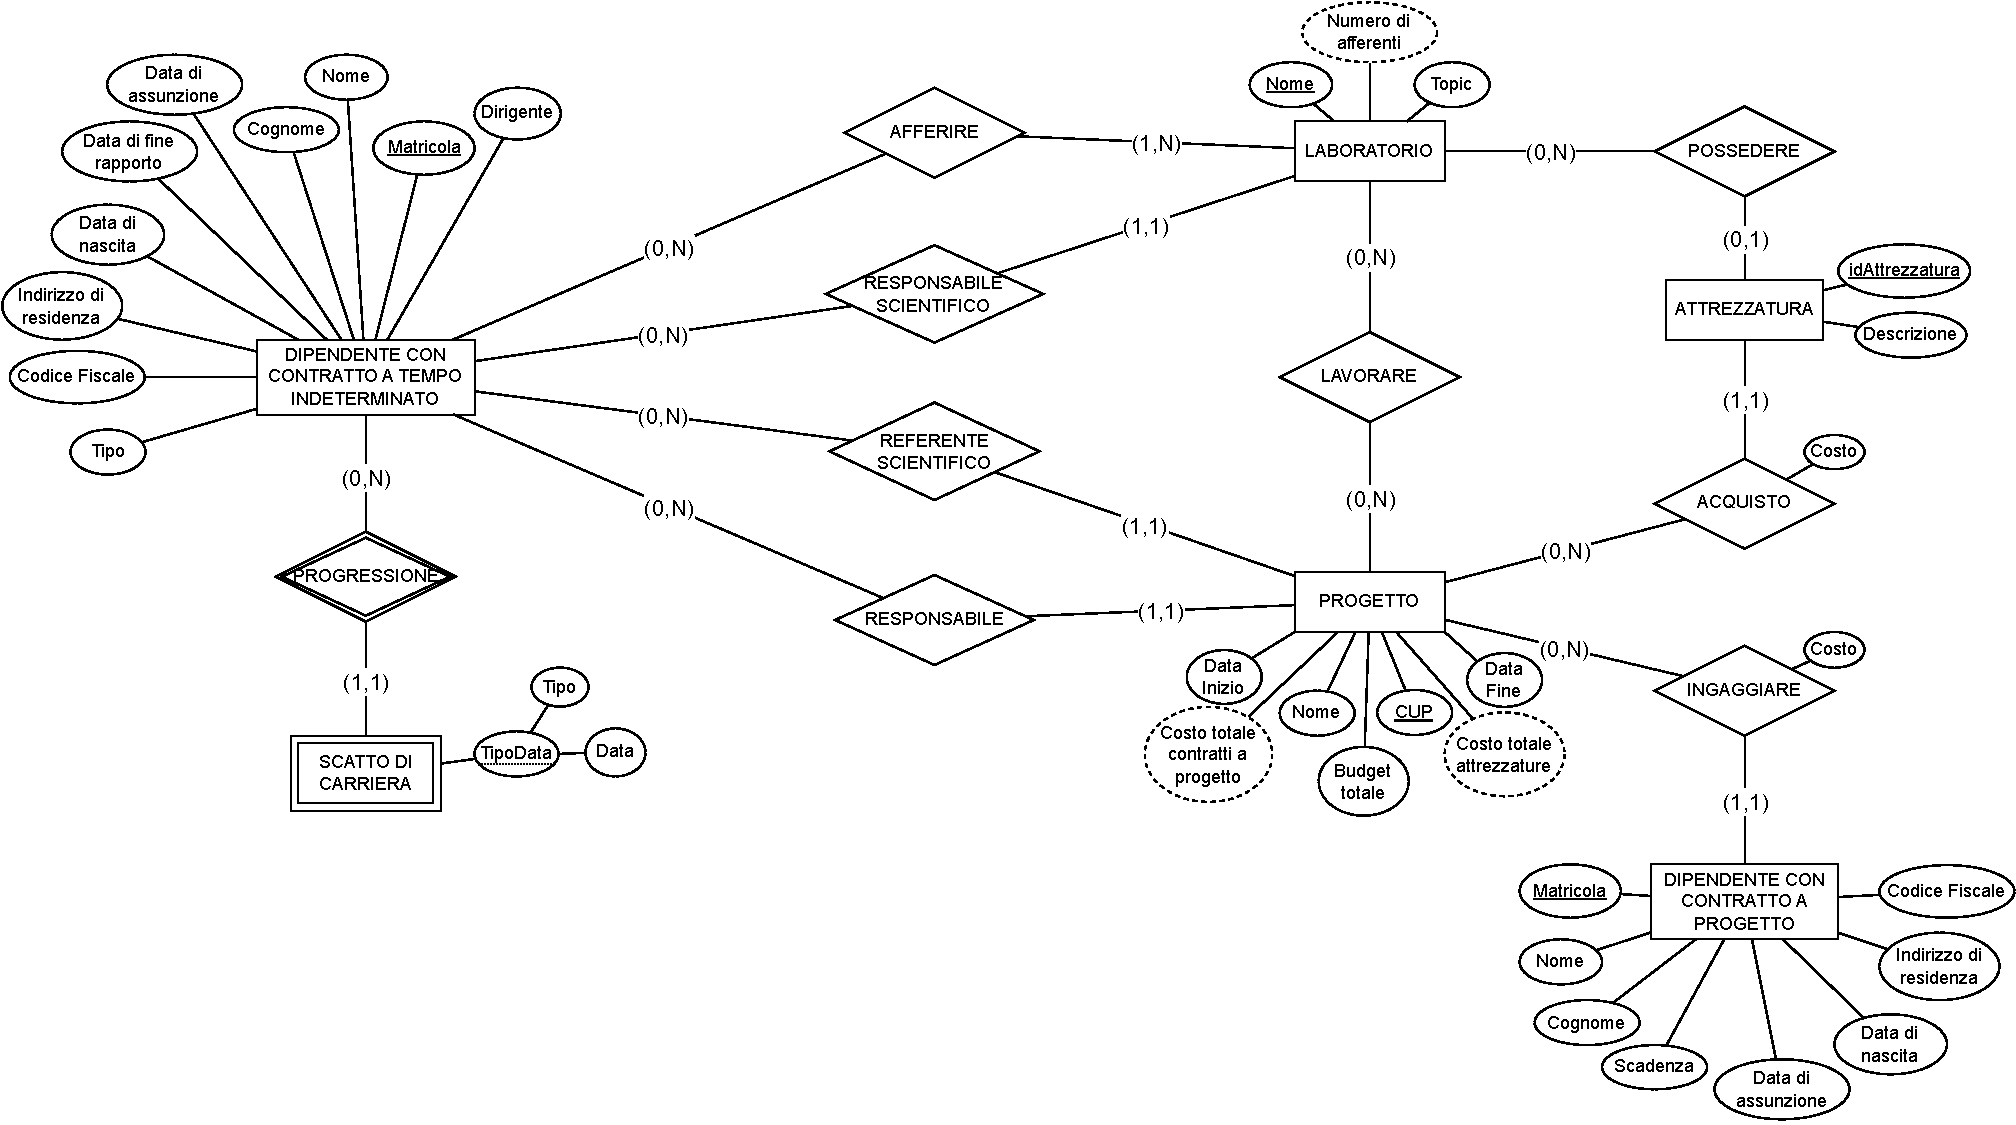
\includegraphics[width=0.85\linewidth]{Diagrammi/Diagramma ER ristrutturato.pdf}
            \caption{Diagramma ER ristrutturato}
            \label{fig:Diagramma ER ristrutturato}
        \end{figure}

    \section{Class Diagram ristrutturato}
        \begin{figure}[htbp!]
            \centering
                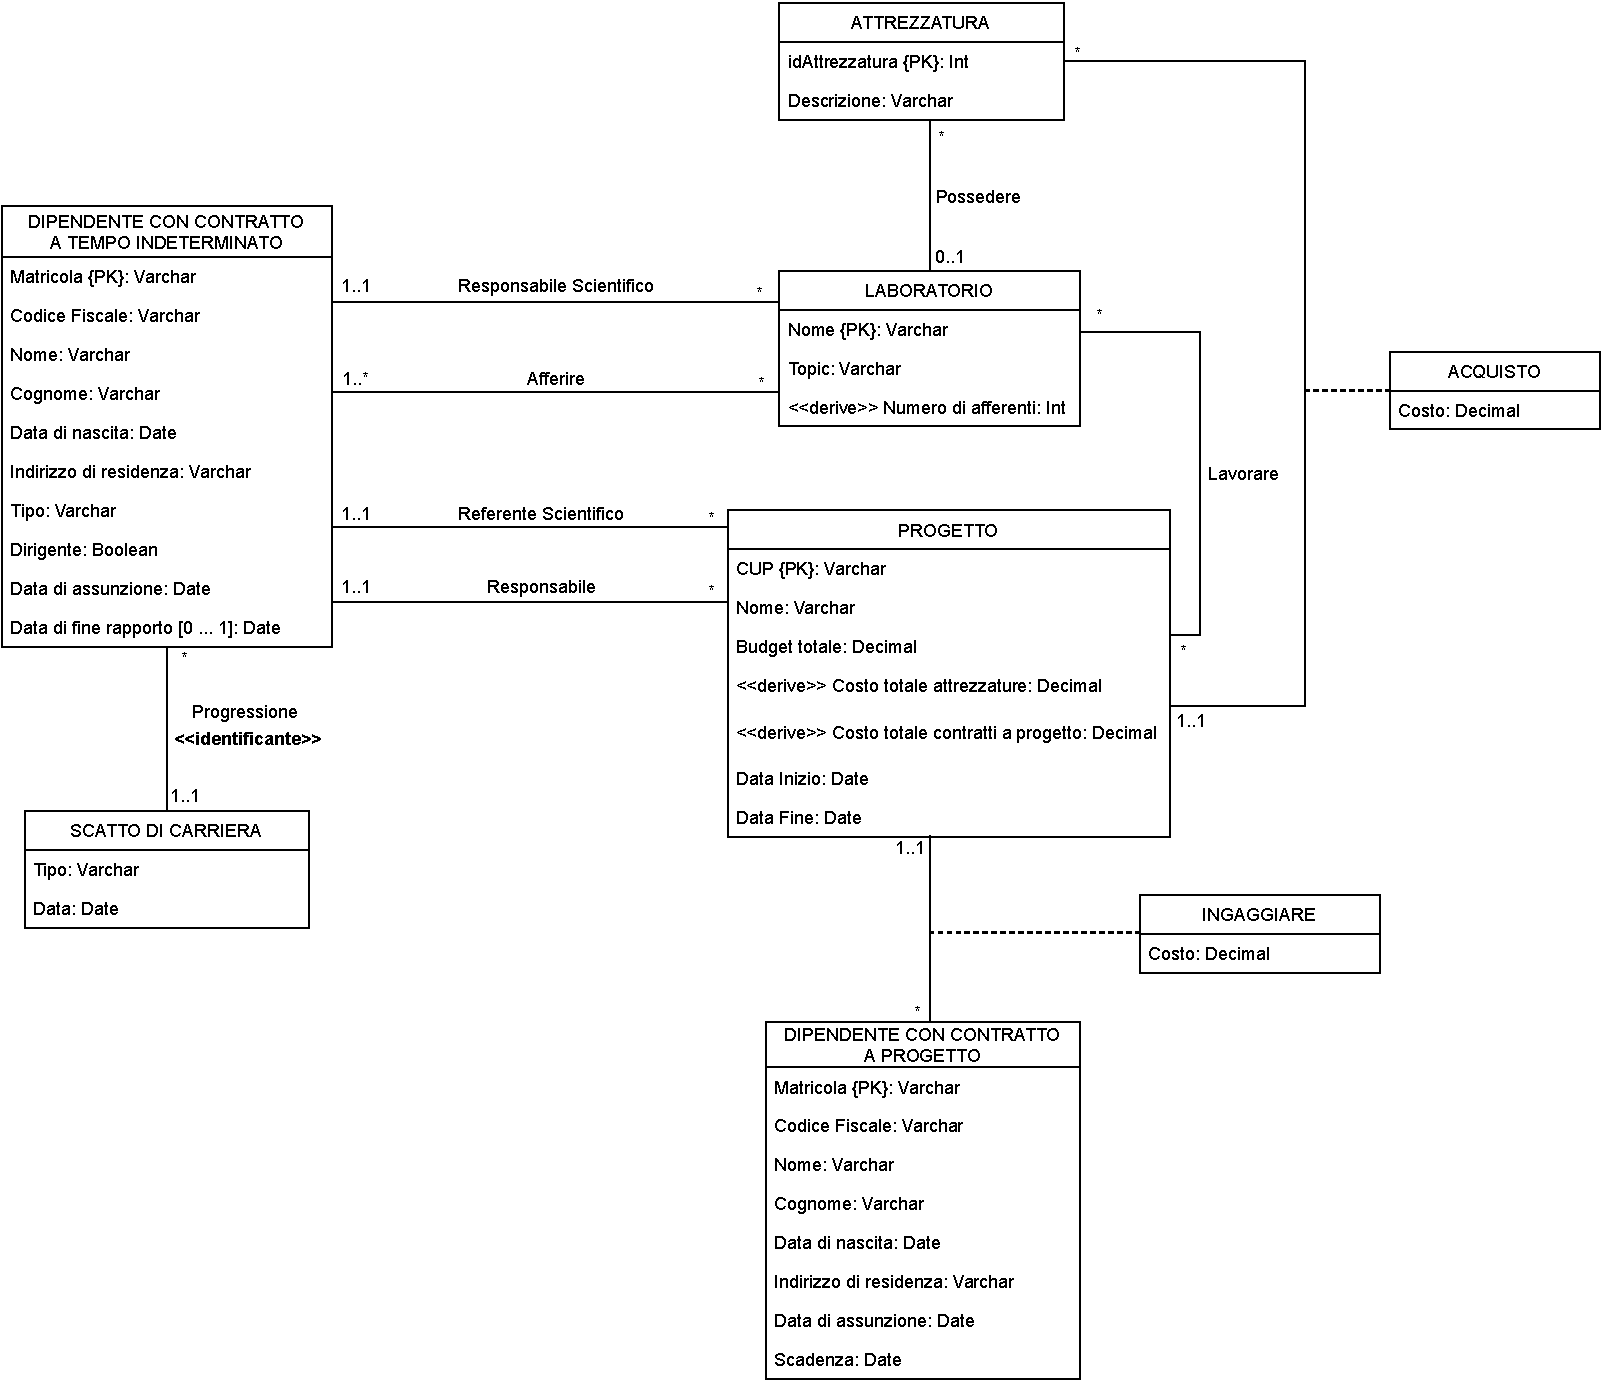
\includegraphics[width=0.67\linewidth]{Diagrammi/Class Diagram ristrutturato.pdf}
            \caption{Class Diagram ristrutturato}
            \label{fig:Class Diagram ristrutturato}
        \end{figure}
    
     \section{Dizionario delle entità}
        \begin{tabular}{|C{3cm}|L{11.7cm}|}
            \hline
            \multicolumn{1}{|c|}{\textbf{Entità}} & \multicolumn{1}{c|}{\textbf{Descrizione}}\\  
            \hline
                DIPENDENTE CON CONTRATTO A TEMPO INDETERMINATO &
                Il tipo di entità "Dipendente con contratto a tempo indeterminato" rappresenta i dipendenti assunti con contratto a tempo indeterminato dall'azienda. Un dipendente con contratto a tempo indeterminato avrà caratteristiche quali: la matricola (unica per ogni dipendente), il nome, il cognome, il codice fiscale, l'indirizzo di residenza, la data di nascita, la data di fine rapporto (ovvero la data in cui eventualmente smette di prestare servizio nell'azienda), la data di assunzione, un attributo tipo che specifica l'anzianità del dipendente (ovvero se è un dipendente junior, middle o senior) e un attributo che indica se il dipendente è attualmente un dirigente o meno.\\
            \hline
                SCATTO DI CARRIERA &
                Il tipo di entità debole "Scatto di carriera" rappresenta gli scatti di carriera di un dipendente. In particolare lo scatto può essere di quattro tipi:
                \begin{enumerate}
                    \item Scatto da junior a middle, indicato con "Middle"
                    \item Scatto da middle a senior, indicato con "Senior"
                    \item Scatto da non dirigente a dirigente, che indichiamo con la denominazione "Promosso a dirigente", non vincolato all'anzianità
                    \item Scatto da dirigente a non dirigente, che indichiamo con la denominazione "Rimosso da dirigente", non vincolato all'anzianità.
                \end{enumerate}
                Oltre al tipo di scatto avremo anche la data in cui è avvenuto lo scatto per una determinata matricola.\\
            \hline
                LABORATORIO &
                Il tipo di entità "Laboratorio" rappresenta i laboratori che si trovano attualmente all'interno dell'azienda. In particolare un laboratorio avrà un nome unico nell'azienda, un topic ed un valore numerico che indica il numero di dipendenti che ad esso afferiscono.\\
            \hline
                ATTREZZATURA &
                Il tipo di entità "Attrezzatura" rappresenta le attrezzature acquistate tramite i fondi di progetti, che possono o meno trovarsi all'interno di un laboratorio. In particolare, un'attrezzatura è un oggetto che avrà un identificativo ed una descrizione (che appunto descrive l'oggetto in questione).\\
            \hline
                PROGETTO &
                Il tipo di entità "Progetto" rappresenta i progetti presi in carico dall'azienda. In particolare il progetto possiederà un CUP (codice unico progetto), un nome, una data di inizio e di fine esecuzione del progetto, il budget totale (che rappresenta i fondi istanziati per quel progetto), il costo totale delle attrezzature acquistate tramite i fondi di quel progetto ed il costo totale dei contratti a progetto dei dipendenti assunti tramite i fondi di quel progetto\\
            \hline
                DIPENDENTE CON "CONTRATTO A PROGETTO" &
                Il tipo di entità "Dipendente con contratto a progetto" rappresenta i dipendenti assunti per lavorare su un progetto tramite un contratto a tempo determinato. Un dipendente con "contratto a progetto" presenterà: una matricola (unica per ogni dipendente), un nome, un cognome, un codice fiscale, un indirizzo di residenza, una data di nascita, una data di assunzione, una data di scadenza (ovvero la data in cui scade il contratto a tempo determinato).\\
            \hline   
        \end{tabular}
        
    \section{Dizionario delle associazioni}
        \begin{tabular}{|C{3cm}|L{11.7cm}|}
            \hline
            \multicolumn{1}{|c|}{\textbf{Associazione}} & \multicolumn{1}{c|}{\textbf{Descrizione}}\\            
            \hline
                PROGRESSIONE &
                L'associazione "PROGRESSIONE" tra "DIPENDENTE CON CONTRATTO A TEMPO INDETERMINATO" e "SCATTO DI CARRIERA" è un'associazione identificante il tipo di entità debole "SCATTO DI CARRIERA", utile per risalire agli scatti di carriera di ogni dipendente. In particolare, un dipendente può avere diversi scatti di carriera, o nessuno. Viceversa, uno scatto è relativo ad un unico dipendente.\\
            \hline
                RESPONSABILE SCIENTIFICO &
                L'associazione "RESPONSABILE SCIENTIFICO" tra "DIPENDENTE CON CONTRATTO A TEMPO INDETERMINATO" e "LABORATORIO" specifica quali dipendenti sono responsabili scientifici di un laboratorio. In particolare, un dipendete potrebbe essere, o meno, Responsabile scientifico di uno o più laboratori. Viceversa, un laboratorio avrà uno ed un solo Responsabile scientifico.\\
            \hline
                AFFERIRE &
                "AFFERIRE" tra "DIPENDENTE CON CONTRATTO A TEMPO INDETERMINATO" e "LABORATORIO" indica quali sono i dipendenti che afferiscono attualmente ad un particolare laboratorio. In particolar modo, un dipendente può afferire a più laboratori, ma potrebbe anche non afferirne a nessuno. Viceversa, un laboratorio può avere più afferenti, oltre al responsabile scientifico.\\
            \hline
                REFERENTE SCIENTIFICO &
                L'associazione "REFERENTE SCIENTIFICO" tra "DIPENDENTE CON CONTRATTO A TEMPO INDETERMINATO" e "PROGETTO" denota quali dipendenti sono referenti scientifici di un progetto. In particolare, un dipendente potrebbe essere, o meno, referente scientifico di uno o più progetti. Al contrario, un progetto deve avere uno ed un solo referente scientifico.\\
            \hline
                RESPONSABILE &
                "RESPONSABILE" tra "DIPENDENTE CON CONTRATTO A TEMPO INDETERMINATO" e "PROGETTO" indica quali dipendenti sono responsabili di un progetto. In particolare, un dipendete potrebbe essere, o meno, responsabile di uno o più progetti, mentre un progetto avrà uno ed un solo responsabile.\\
            \hline
                LAVORARE &
                L'associazione "LAVORARE" tra "LABORATORIO" e "PROGETTO" fa corrispondere, ad ogni laboratorio, i progetti a cui ha lavorato. In particolare, un laboratorio può aver lavorato a più progetti, così come potrebbe non aver mai lavorato ad alcun progetto. Viceversa, un progetto presenta dei laboratori che lavorano ad esso, oppure nessuno.\\
            \hline
                POSSEDERE &
                "POSSEDERE" tra "LABORATORIO" e "ATTREZZATURA" indica le attrezzature appertenenti ad un laboratorio. Un laboratorio potrebbe avere più attrezzature, così come potrebbe non averne nessuna. All'opposto, un'attrezzatura appartiene, o meno, ad un laboratorio.\\
            \hline
                ACQUISTO &
                "ACQUISTO" tra "ATTREZZATURA" e "PROGETTO" fornisce informazioni circa le attrezzature acquistate tramite i fondi di un progetto, infatti ogni acquisto avrà un costo. Dunque, sarà possibile acquistare più attrezzature, o nessuna, per un progetto. Invece, tutte le attrezzature devono essere acquistate tramite i fondi di uno ed un solo progetto.\\
            \hline
                INGAGGIARE &
                L'associazione tra "PROGETTO" e "DIPENDENTE CON CONTRATTO A PROGETTO" denominata "INGAGGIARE" indica quali sono i dipendenti ingaggiati utilizzando il budget di un progetto, ed ogni ingaggio di un nuovo contratto avrà un costo. Infatti, sarà possibile ingaggiare più dipendenti con contratto a progetto, o nessuno. Viceversa, un dipendente con contratto a progetto, se presente, è stato assunto mediante i fondi di uno ed un solo progetto.\\
            \hline
        \end{tabular}
